
\documentclass{article}
\usepackage[spanish]{babel} %Definir idioma español
\usepackage[utf8]{inputenc} %Codificacion utf-8
\usepackage{amssymb, amsmath, amsbsy, wasysym}
\usepackage{multirow} % para tablas
\usepackage{graphicx}
\title{Práctica 2\\Redes de computadoras}
\author{Emmanuel Peto Gutiérrez}
\begin{document}
\maketitle

\section{Pasos para realizar la práctica}

El primer paso es iniciar sesión en AWS e ir a la consola. Se busca el servicio VPC y se elige alguna región disponible (en mi caso solo Virginia).

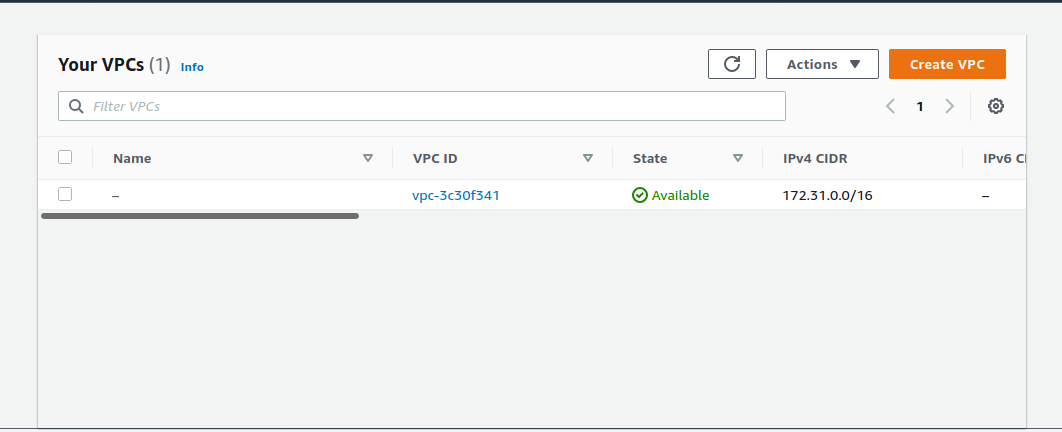
\includegraphics[width=\linewidth]{imagenes/paso1}

También se busca el servicio EC2.

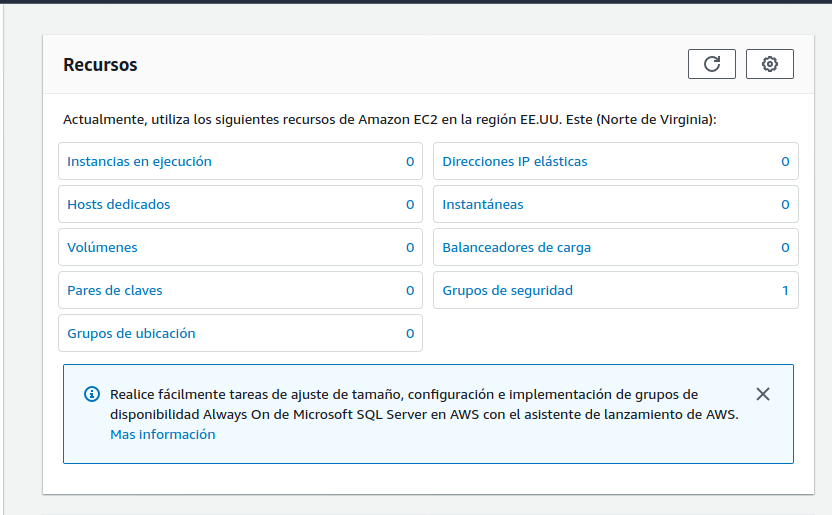
\includegraphics[width=\linewidth]{imagenes/paso2}

En la pantalla de EC2 se busca un botón naranja que dice ``Lanzar la instancia''; hay que pinchar ese botón. En la página a la que se dirige hay que buscar Ubuntu 20 y presionar el botón select.

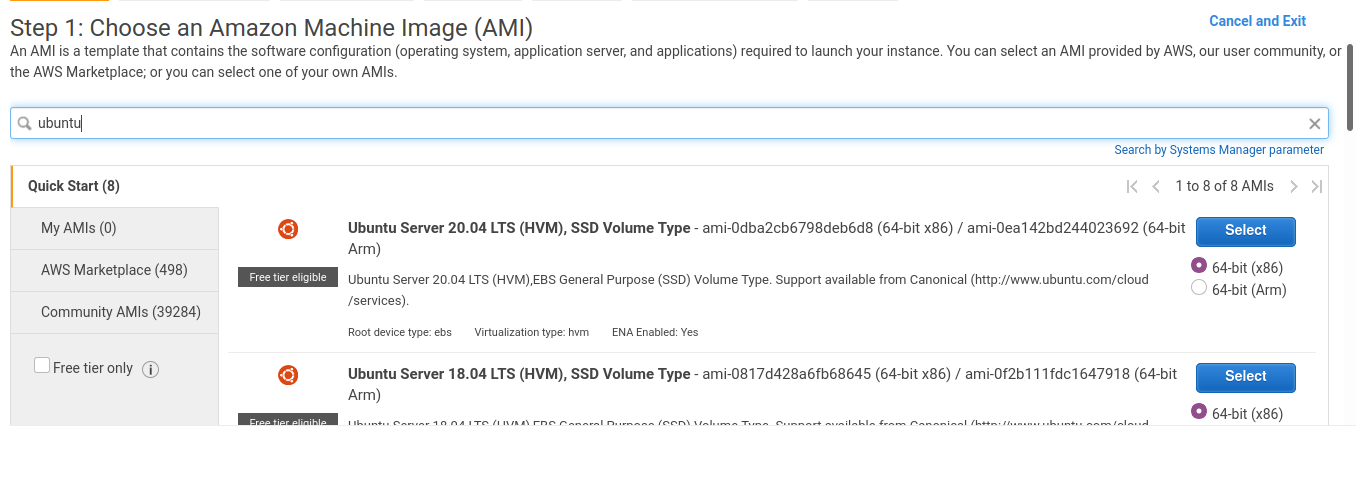
\includegraphics[width=\linewidth]{imagenes/paso3}

Nos enviará a una pantalla donde se elige el tamaño del servicio. Se eligió la micro porque dice \textit{free tier eligible}. Luego se presiona el botón \textit{Next: Configure Instance Details}

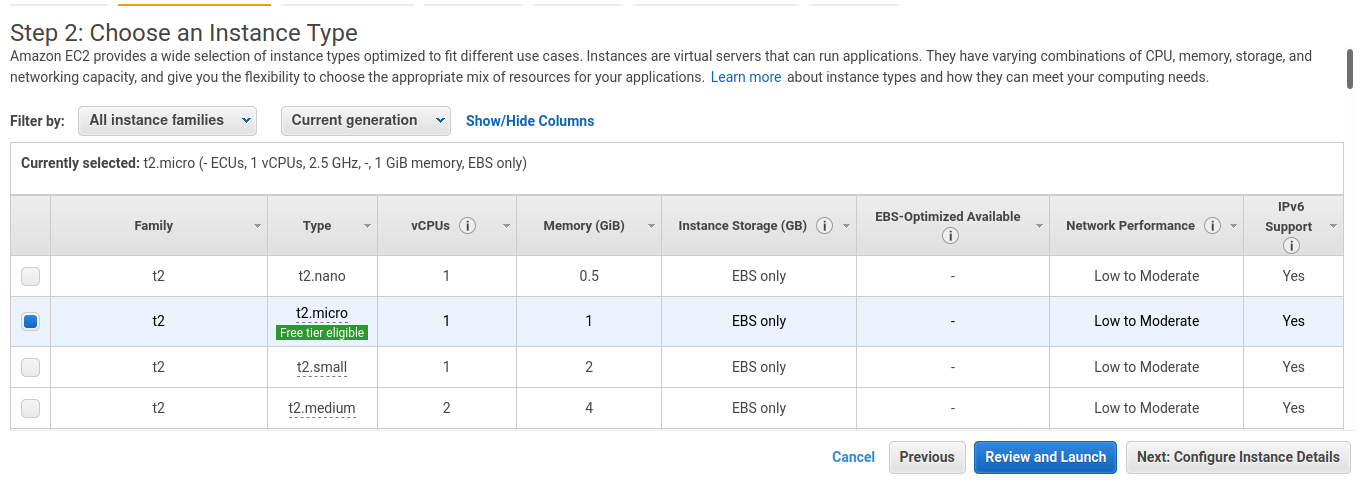
\includegraphics[width=\linewidth]{imagenes/paso4}

En esta pantalla, en la opción \textit{Network}, el nombre del VPC debe ser el mismo que el del VPC que se acaba de crear. Se presiona el botón \textit{Next: Add Storage}

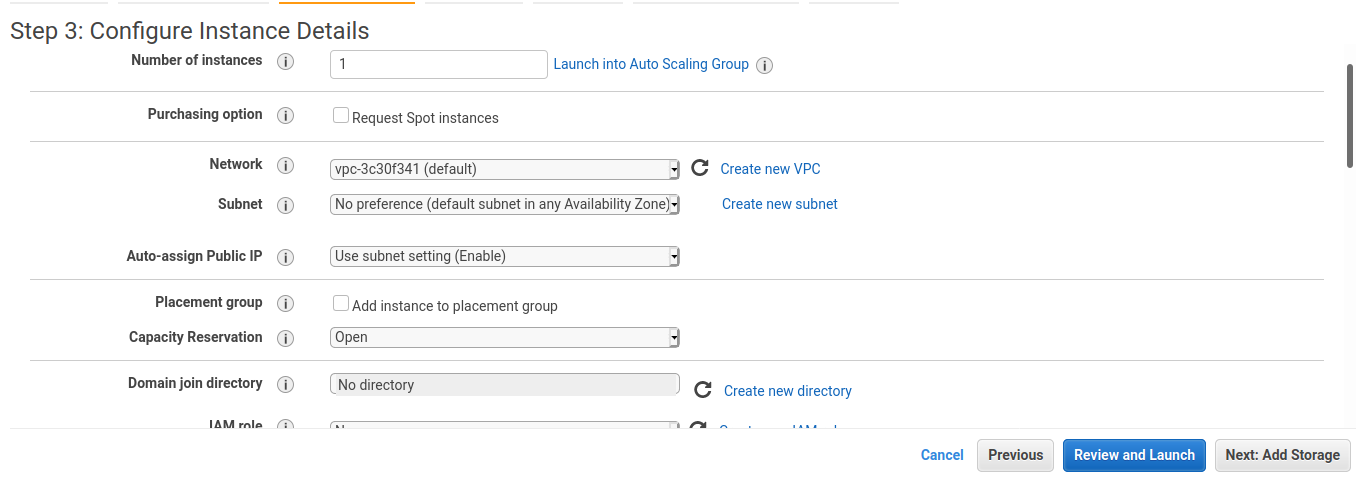
\includegraphics[width=\linewidth]{imagenes/paso5}

En el almacenamiento se dejan todas las opciones por defecto y se presiona \textit{Next: Add Tags}.

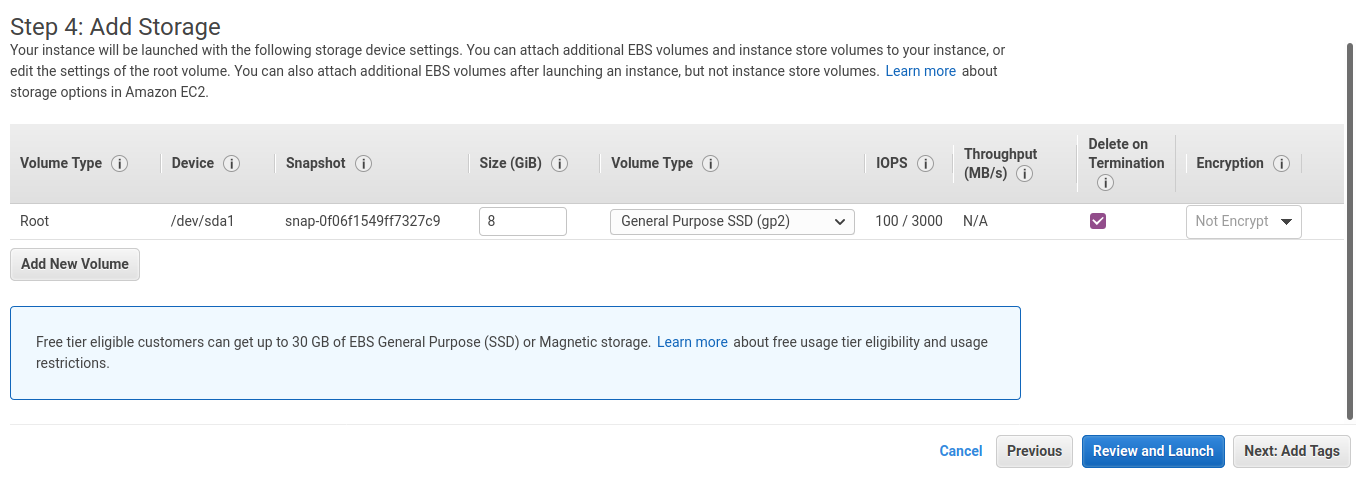
\includegraphics[width=\linewidth]{imagenes/paso6}

En la siguiente pantalla se presiona el botón \textit{Add Tag}. La llave de la etiqueta es \textbf{Redes} y el valor es \textbf{practica2}. Luego se presiona \textit{Next: Configure Security Group}.

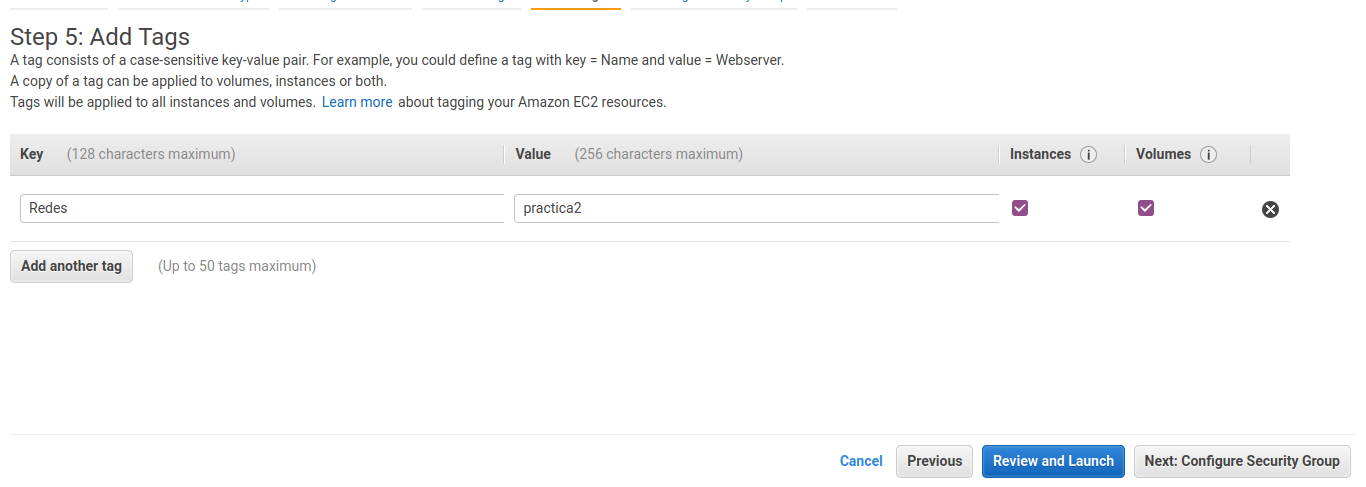
\includegraphics[width=\linewidth]{imagenes/paso7}

En la seguridad se añade una nueva regla: el tipo HTTP. Después se presiona \textit{Review and Launch}.

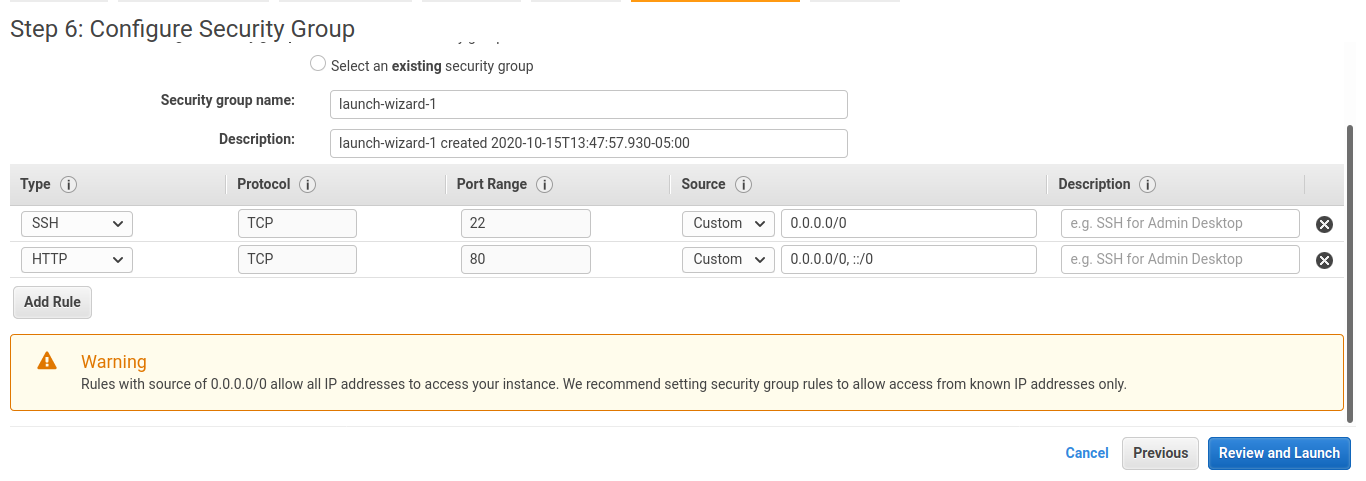
\includegraphics[width=\linewidth]{imagenes/paso8}

En la siguiente página solo se presiona \textit{Launch}.

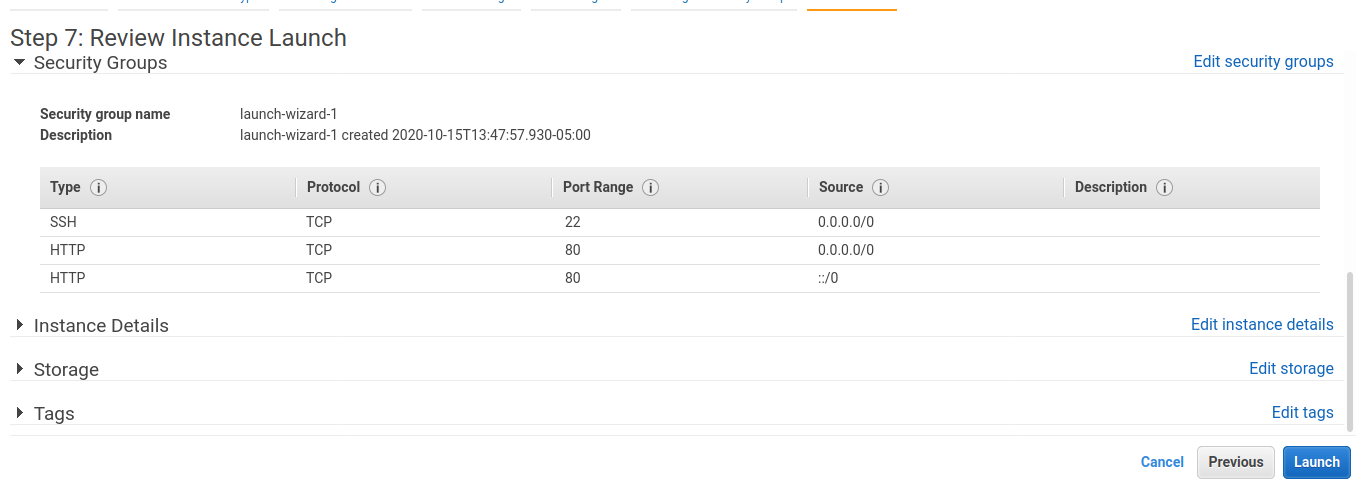
\includegraphics[width=\linewidth]{imagenes/paso9}

Se creó un par de llaves y se descargó el archivo .pem. Después se dió al botón \textit{Launch Instances}.

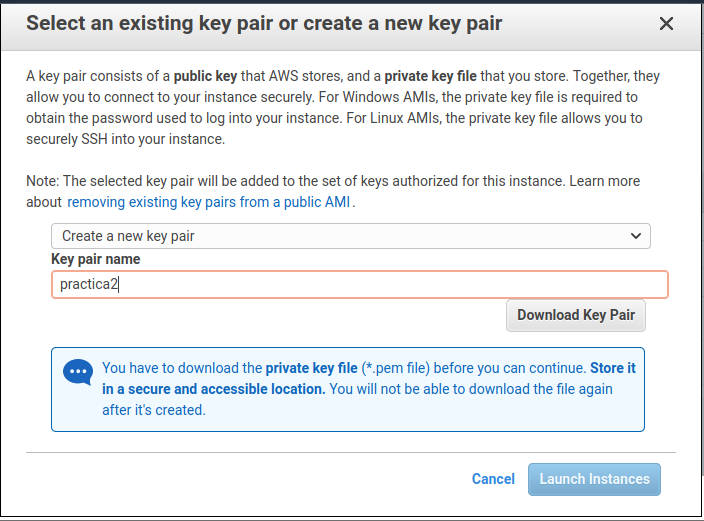
\includegraphics[width=\linewidth]{imagenes/paso10}

En esta pantalla hay que buscar el botón \textit{View instances} que está hasta abajo.

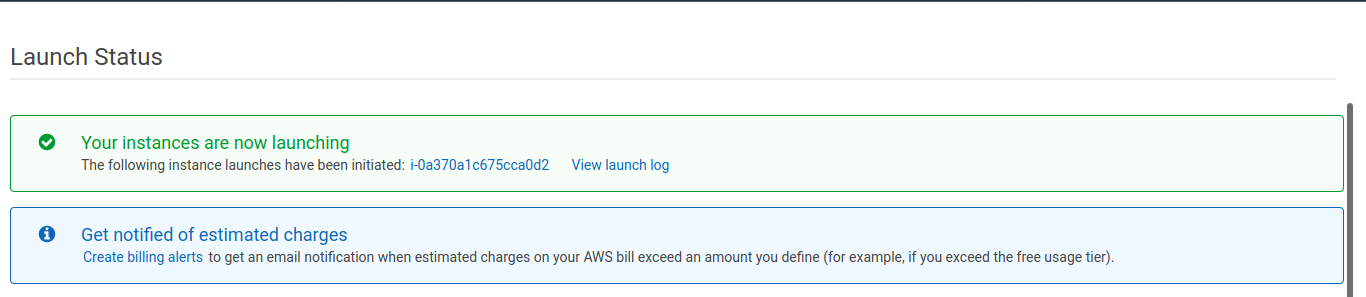
\includegraphics[width=\linewidth]{imagenes/paso11}

Y listo, la instancia está en ejecución.

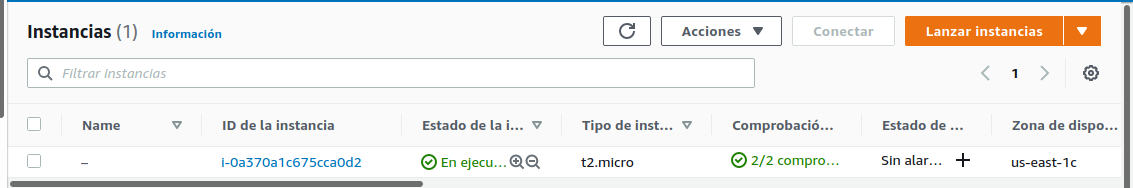
\includegraphics[width=\linewidth]{imagenes/paso12}

Una vez descargada la llave (practica2.pem), se colocó en el directorio home de mi equipo. Aquí se cambian los permisos del archivo con \texttt{chmod}.

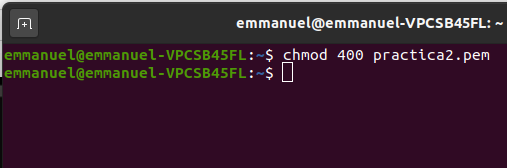
\includegraphics[width=\linewidth]{imagenes/paso13}

Luego, en los detalles de la instancia se dio click al botón \textit{Conectar}.

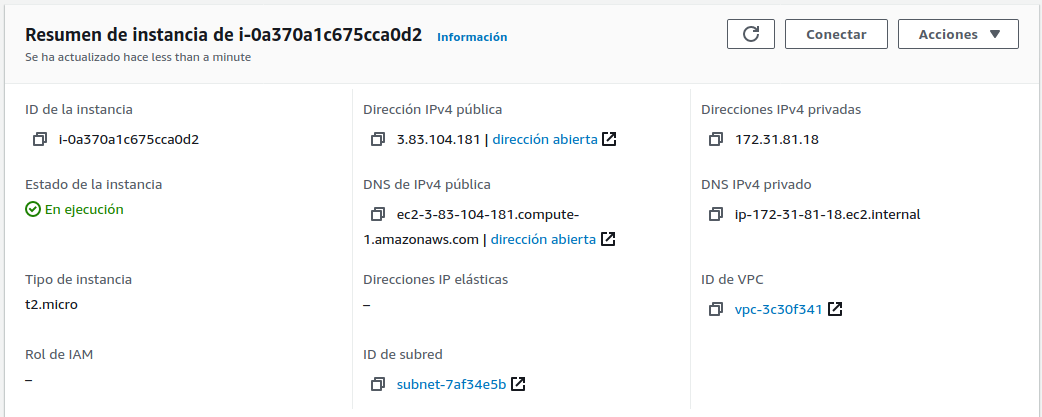
\includegraphics[width=\linewidth]{imagenes/paso14}

En la pestaña Cliente SSH se dan instrucciones para conectarse mediante SSH. Se debe colocar en la consola de nuestra computadora el comando que viene después de ``Ejemplo:''

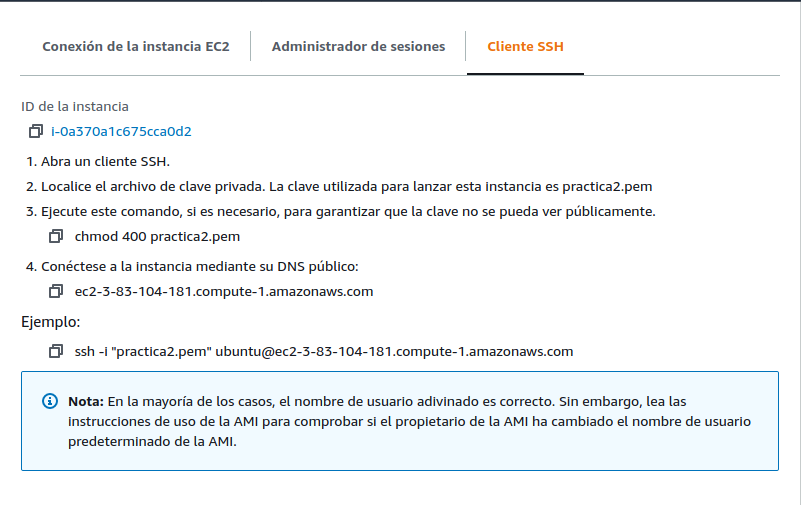
\includegraphics[width=\linewidth]{imagenes/paso15}

Después hay que escribir ``yes'' y se conecta.

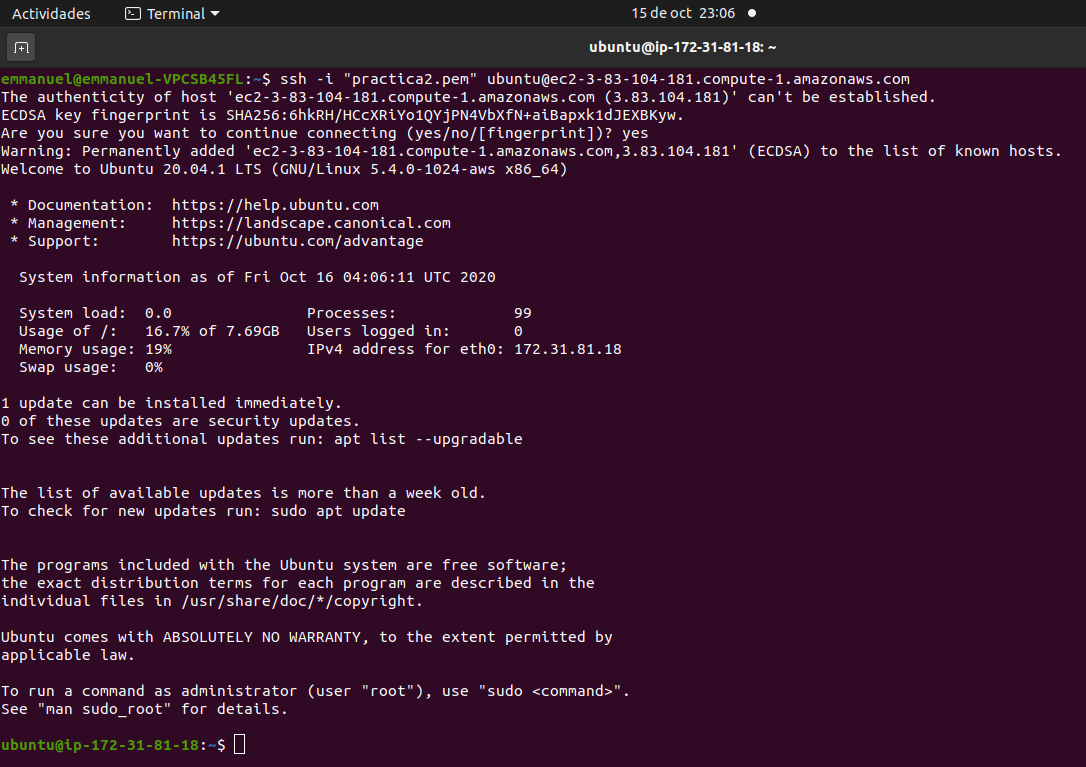
\includegraphics[width=\linewidth]{imagenes/paso16}

Una vez conectado al servidor, se actualiza la lista de paquetes con \texttt{sudo apt update}.

Luego, hay que instalar apache con \texttt{sudo apt install apache2}.

Para ver las conexiones actuales al servidor se ejecuta \texttt{sudo ss -nat}.

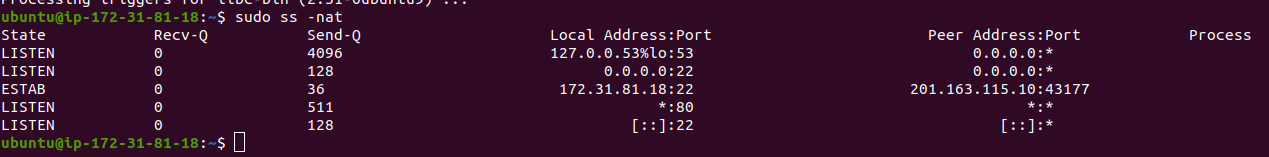
\includegraphics[width=\linewidth]{imagenes/paso17}

Para entrar al servidor mediante HTTP se coloca la IP pública en un navegador.

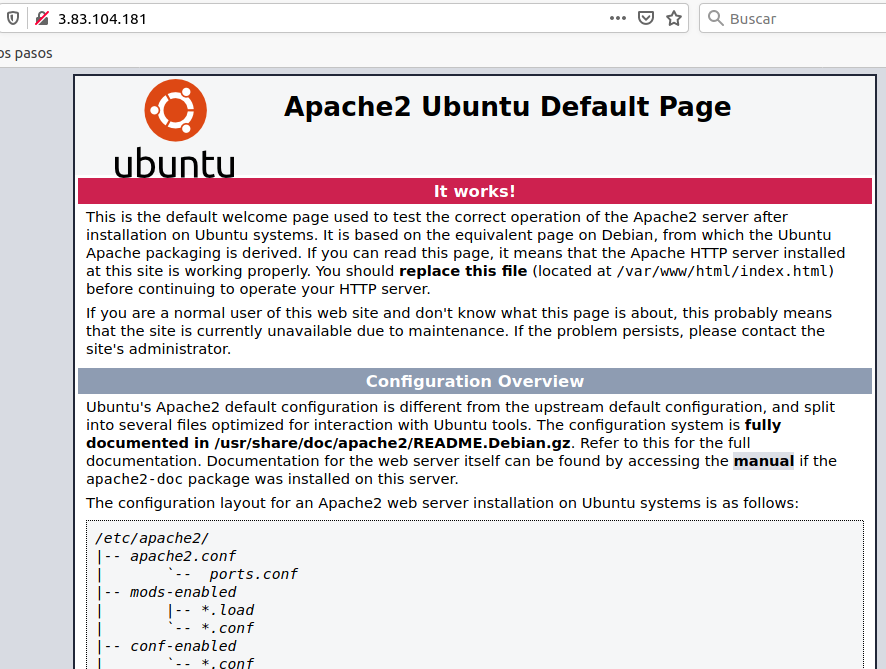
\includegraphics[width=\linewidth]{imagenes/paso18}

Se cambia de dirección a \texttt{/var/www/html}. Después, se ven los archivos en ese directorio con \texttt{ls -l}. Ya existe ahí un archivo \texttt{index.html}, el cual se procede a borrar con \texttt{sudo rm index.html}.

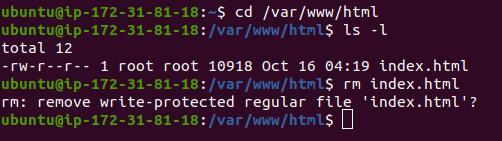
\includegraphics[width=\linewidth]{imagenes/paso19}

Se crea y abre un archivo nuevo con \texttt{sudo vi index.html}. En esta parte se creó una página html que contiene un formulario.

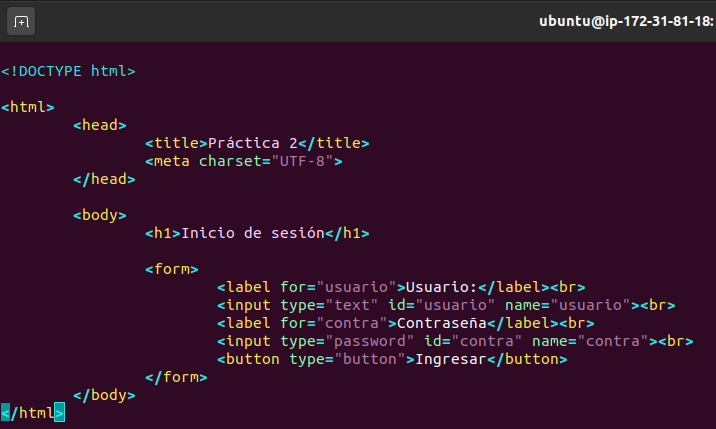
\includegraphics[width=\linewidth]{imagenes/paso20}

Regresando a AWS, nos vamos a la sección de \textit{Red y seguridad/Direcciones IP elásticas} del lado izquierdo de la página. En esta página aparece un botón naranja que dice \textit{Asignar la dirección IP elástica}.

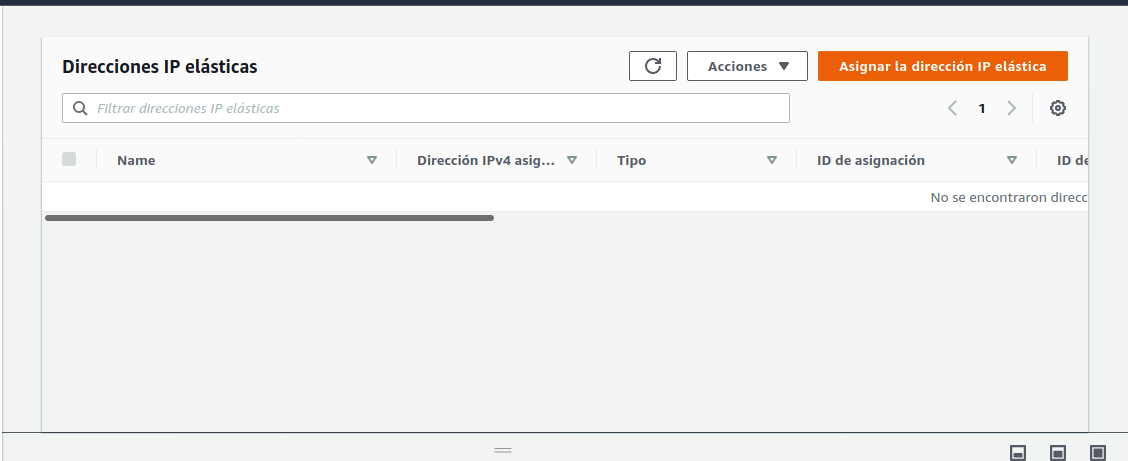
\includegraphics[width=\linewidth]{imagenes/paso21}

Aquí solo hay que presionar el botón \textit{Asignar}.

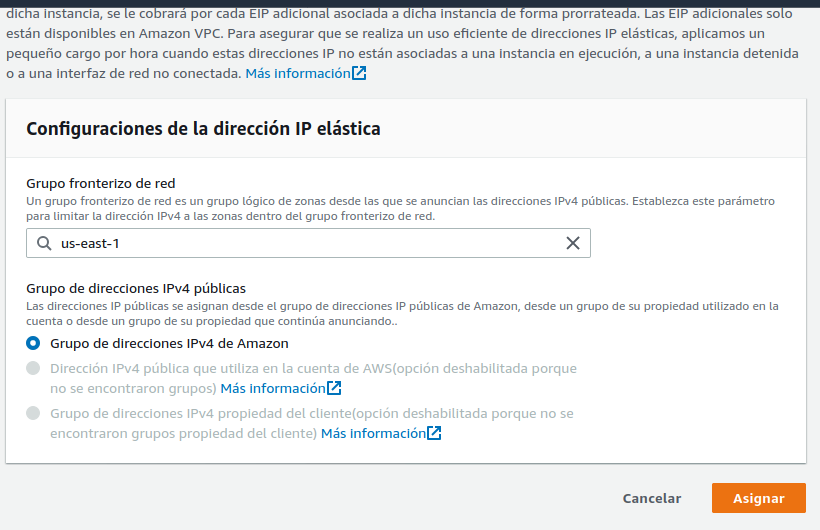
\includegraphics[width=\linewidth]{imagenes/paso22}

En la parte de arriba, en la barra verde, está el botón \textit{Asociar esta dirección IP elástica}. Hay que pinchar ese botón.

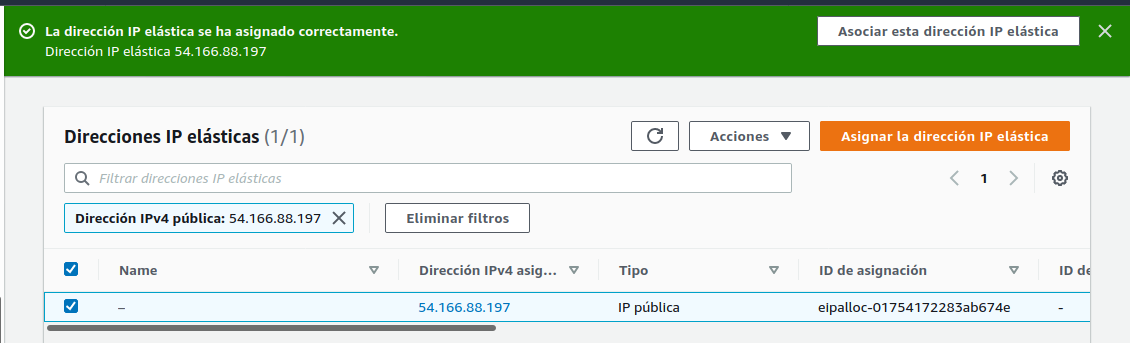
\includegraphics[width=\linewidth]{imagenes/paso23}

Luego, hay que asociar la dirección IP elástica con la instancia de Ubuntu que acabamos de crear (debajo de la etiqueta \textit{Instancia}). Hay que marcar el checkbox que dice \textit{Permitir que se vuelva a asociar esta dirección IP elástica}. Por último, hay que pinchar el botón de \textit{Asociar}.

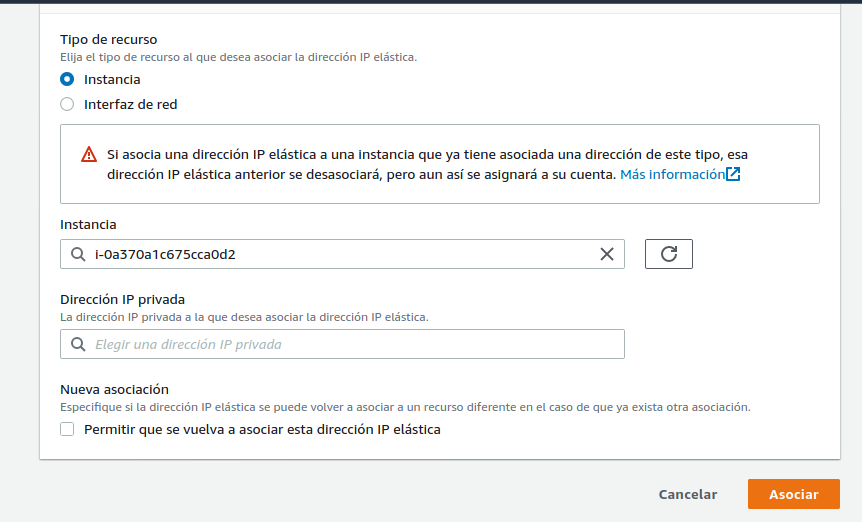
\includegraphics[width=\linewidth]{imagenes/paso24}

Debería aparecer una notificación de que la dirección IP elástica ya está asociada.

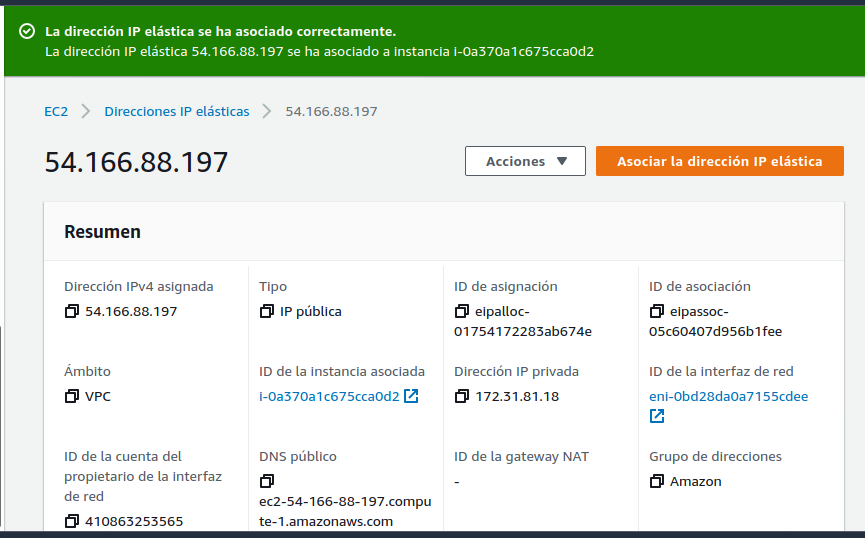
\includegraphics[width=\linewidth]{imagenes/paso25}

Se puede comprobar que esa dirección IP está asociada a la instancia poniendola en el navegador. Debería aparecer la página que se acaba de crear con HTML.

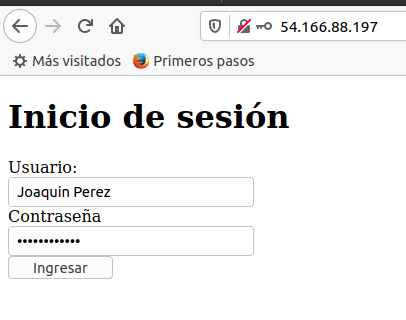
\includegraphics[width=\linewidth]{imagenes/paso26}

Para finalizar, hay que detener la instancia. En \textit{Detalles de la instancia} hay que ir a \textit{Acciones/Detener instancia}.

\section{Cuestionario}

\textbf{1. ¿Qué es el concepto de nube y a qué se refiere el término Iaas? (describir con sus propias palabras aunque sea un renglón).}

La \textit{nube} es un conjunto de servidores remotos destinados a proveer servicios a las personas o empresas. Los servicios pueden ser: guardar archivos, ejecutar aplicaciones web, cómputo distribuido, et al.

El IaaS es la interfaz entre los usuarios de servicios en la nube y la infraestructura de los servidores remotos. Amazon Web Services es un ejemplo.\\

\textbf{2. ¿Qué ventajas observas al utilizar la infraestructura que utilizamos en esta práctica? (describir con sus propias palabras aunque sea un renglón).}

En caso de que una persona o empresa necesite montar una aplicación web de manera rápida, no es necesario invertir en la infraestructura inicialmente para montarla; simplemente necesita contratar los servicios del IaaS para montarla. También puede dar de baja rápidamente su aplicación si ya no la va a utilizar.\\

\textbf{3. Colocar comentarios sobre la práctica (facilidad de ejecución, valoración de lo aprendido).}

Seguir instrucciones fue relativamente fácil, excepto porque a veces ocurrían errores inesperados relacionados con AWS que no le pasaban al profesor. En mi caso, tuve que esperar 4 horas a que verificaran si tenía permiso de crear una instancia.

\end{document}

